\documentclass{beamer}
\usepackage{beamerthemeshadow}
\usepackage{graphicx}
\graphicspath{{./slike/}}
\usepackage{color}
\usepackage[utf8]{inputenc}
\usepackage[T2A]{fontenc}
\usepackage{hyperref}
\usepackage[flushleft]{threeparttable}
\definecolor{beamer@darkred}{rgb}{0.1,0.85,0.4}
\setbeamercolor{structure}{fg=beamer@darkred}

\title{Сајбер криминал и мере заштите}
\subtitle{Семинарски рад у оквиру курса Техничко и научно писање}
\author{Богдан Мицић, \\Никола Милорадовић, \\Исидора Перовић, \\Филип Антанасковић}
\institute{Математички факултет\\Универзитет у Београду}
\date{
  \footnotesize{10.12.2022.}
}
%литература и насловна страна иду изнад
%када пишете имаћемо два section-a: Filipov i moj deo, dok Isidora i Nikola kada budu pisali svoj treba da koriste \subsection, razlog jer po pravilu u pregledu ne bi trebali da imamo vise od 3 glavne teme tj. sectiona
\begin{document}

\begin{frame}
  \thispagestyle{empty}
  \titlepage{}
\end{frame}
\addtocounter{framenumber}{-1}

\begin{frame}[fragile]\frametitle{Литература}
  \begin{itemize}
    \item В. Кораћ, Д. Прља, А. Дилигенски, \emph{Дигитална форензика}, Београд 2016.
    \item Сајбер тероризам као окидач све интензивније потребе за безбедност система од опасности које долазе са интернета, Сандра Клисарић, 2021.
    \item Eric Cole, \emph{How to secure your company}, Computerworld, 2016.
    \item Ханипот и где се користи, \url{https://www.kaspersky.com/resource-center/threats/what-is-a-honeypot}
    \item Вештачка интелигенција у сигурносним системима, \url{https://vectra.ai/learning/ai-security2}
  \end{itemize}
\end{frame}

\begin{frame}
	\frametitle{Преглед}
	\tableofcontents
\end{frame}
\section{Сајбер криминал}

\begin{frame}\frametitle{Увод: о сајбер криминалу}
  \begin{itemize}
    \item Мотиви за сајбер криминал:
    \begin{itemize}
      \item крађа и продаја података
      \item шпијунажа
      \item бесплатно коришћење програма и мултимедијалних садржаја
    \end{itemize}
    \item Стање сајбер криминала:
    \begin{itemize}
      \item већина великих организација је претрпела сајбер нападе
      \item IDS (Intrustion Dectection System) системи нису решили проблеме
      \item велики број умрежених рачунара за дистрибуцију пиратерије
      \item сајбер криминал је статистички најдоминантнији тип криминала
    \end{itemize}
  \end{itemize}
\end{frame}

\begin{frame}\frametitle{Пораст коришћења интернета у свету током година}
  \begin{figure}[h]
  \centering
  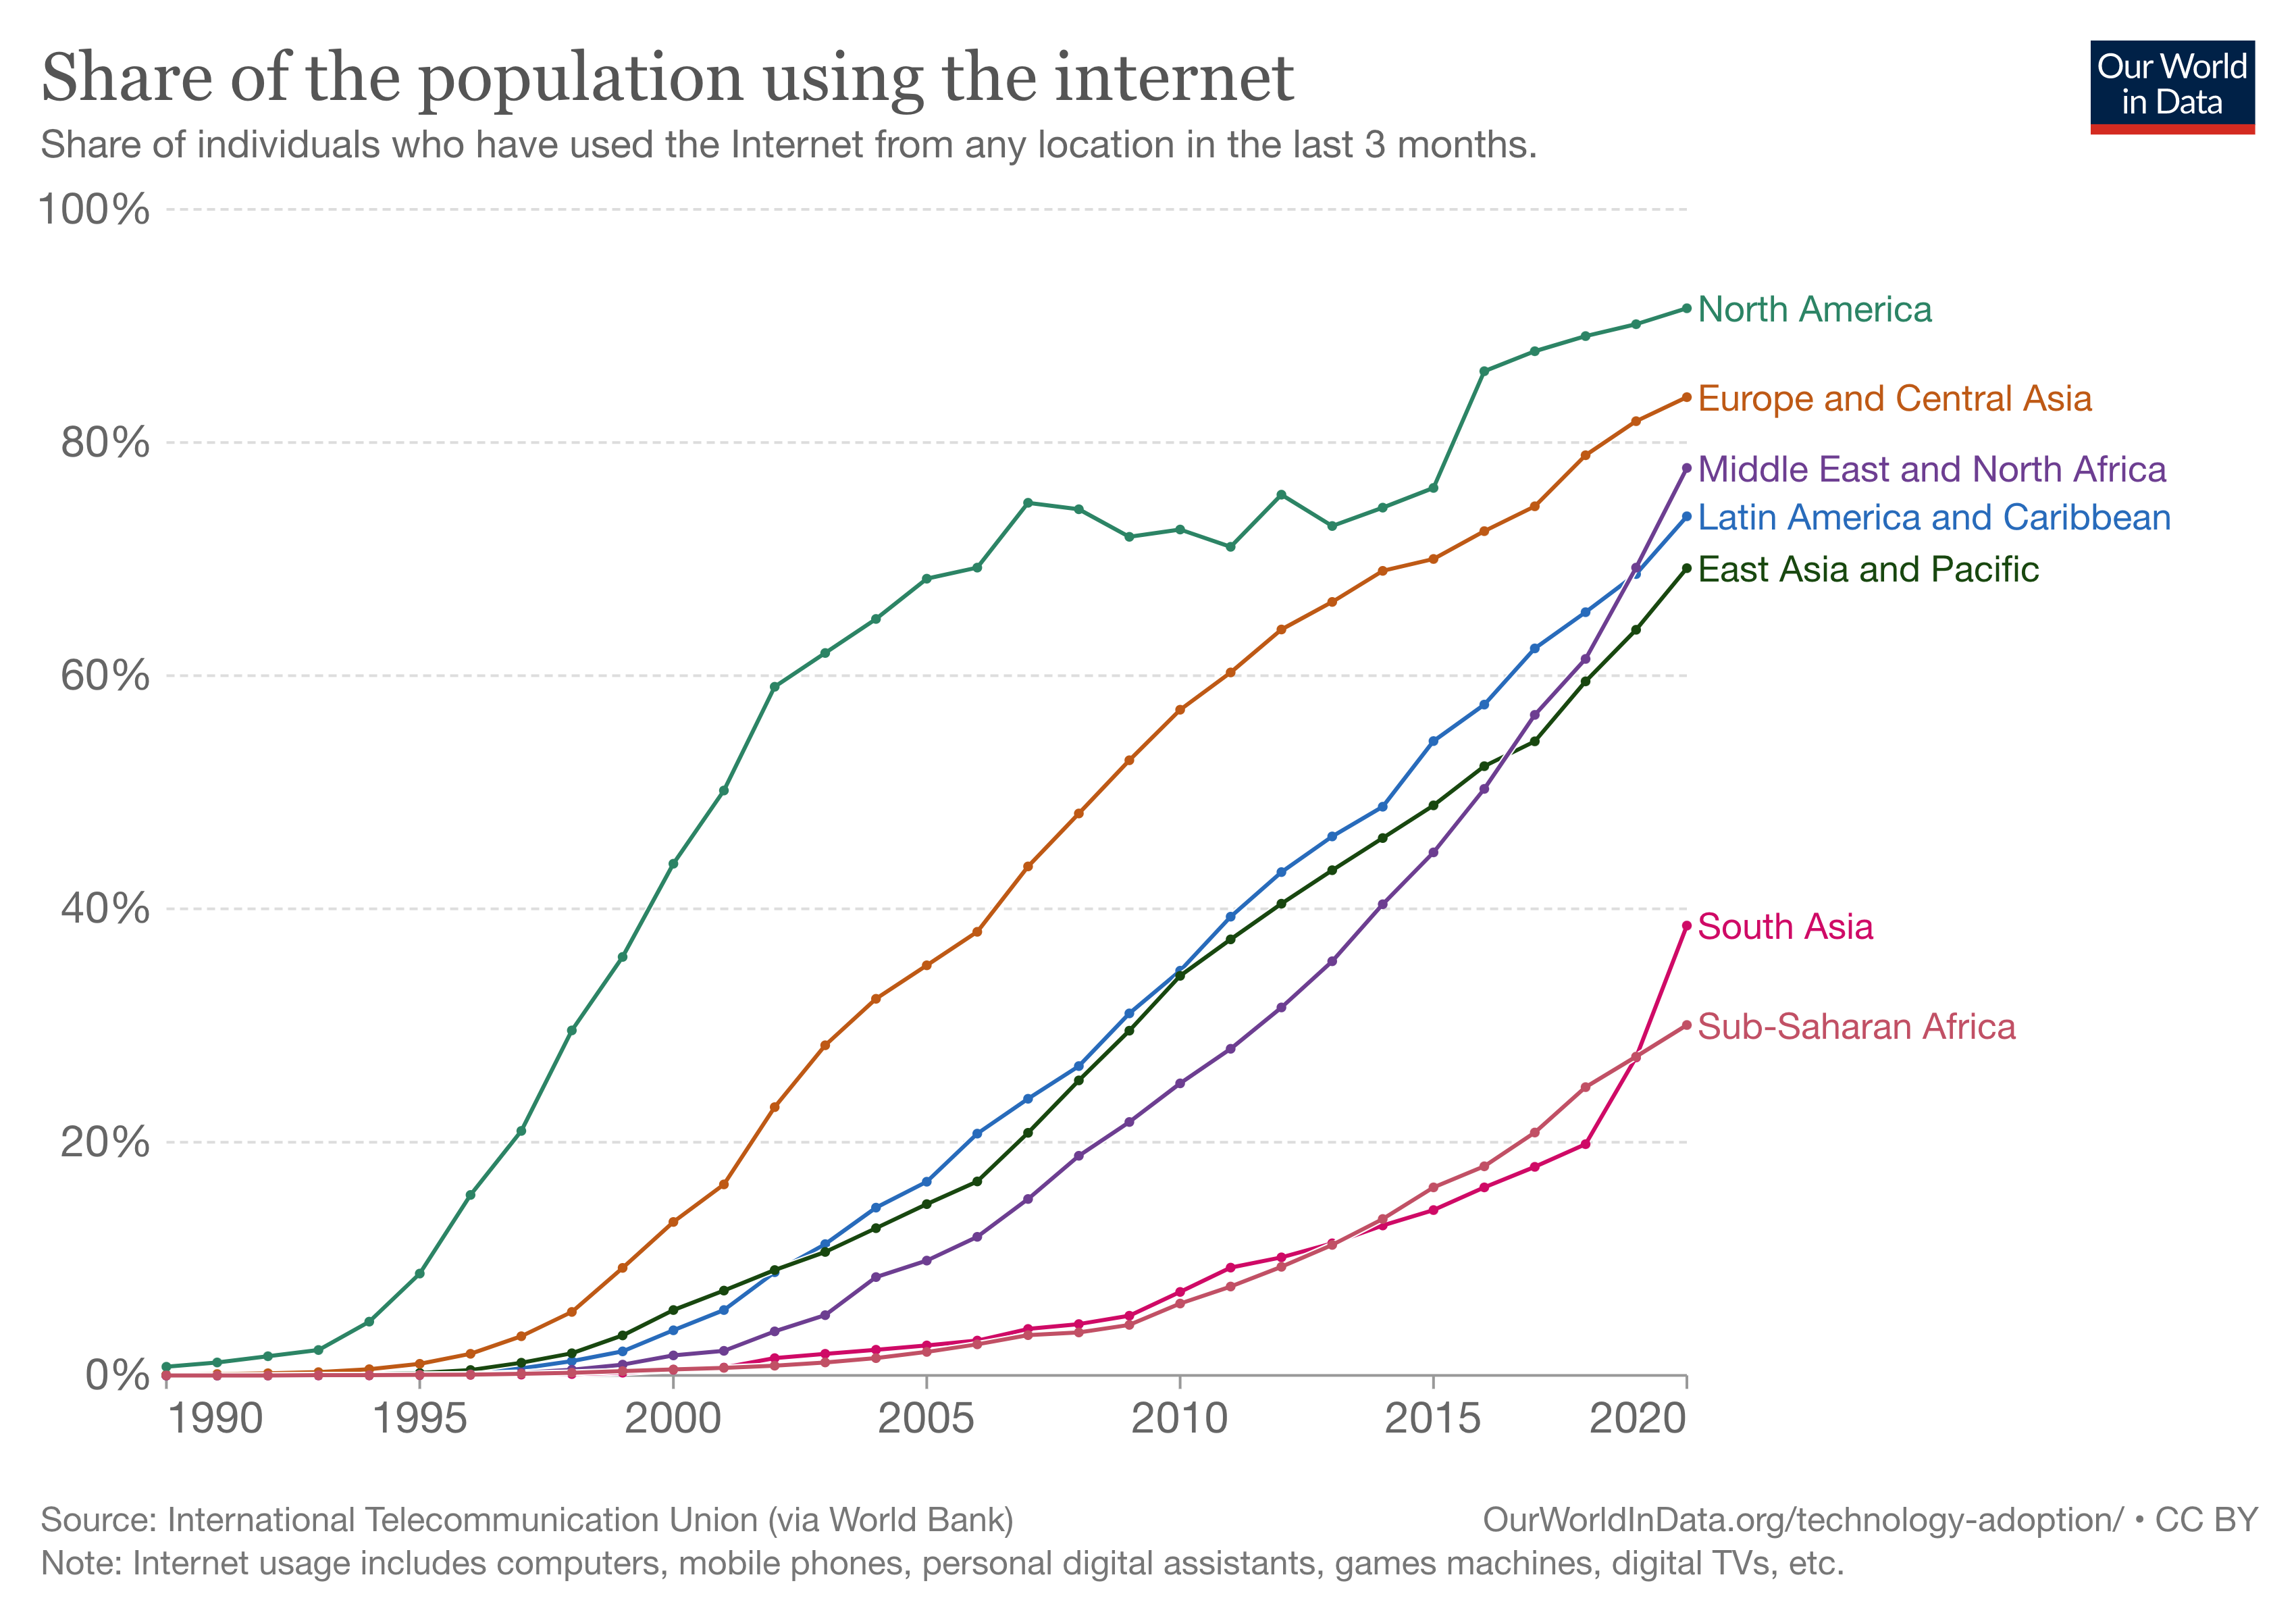
\includegraphics[width=1.0\textwidth]{koriscenje-interneta-po-godinama.png}
  \end{figure}
\end{frame}

\subsection{Типови сајбер криминала}

\begin{frame}\frametitle{Типови сајбер криминала}
	\begin{itemize}
		\item Типови сајбер криминала:
		\begin{itemize}
			\item Сајбер криминал у ужем смислу
			\item Сајбер криминал у ширем смислу
		\end{itemize}
		\item Конкретни облици сајбер криминала:
		\begin{itemize}
			\item Неовлашћен приступ
			\item Оштећење података или програма
			\item Неовлашћено пресретање комуникација
			\item Саботажа
			\item Шпијунажа
		\end{itemize}
		\item Учиниоци дела сајбер криминала:
		\begin{itemize}
			\item Злонамерни учиниоци
			\item Учиниоци не мотивисани проузроковањем штете
		\end{itemize}
	\end{itemize}  
\end{frame}

\subsection{Примена у пракси}

\begin{frame}[fragile]\frametitle{Примена у пракси}
	\begin{itemize}
		\item Владимир Левин, софтверски инжењер из Петрограда, краде 10 милиона долара из Citybank-а
		\item ,,Црв" Морис 1998. године
		\item Џонатан Џозеф Џеjмс упада у Агенцију Министарства Одбране и НАСУ 1999.
		\item 2003. године црв наноси штету од 1.2 милијарде долара
		\item Украjинска криминална организациjа фалсификује кредитне картице 2009.
		\item Случај AshleyMadison.com 
		\item Авионски инцидент 2015. године
	\end{itemize}
\end{frame}

%сви остали делови иду изнад мог
\section{Мере заштите}

\begin{frame}[fragile]\frametitle{Мере заштите}
	\begin{itemize}	
	\item Мере заштите које могу применити појединци
		\begin{itemize}
		\item опрезност на интернету
		\item редовно ажурирање оперативног система и антивирусног софтвера
		\item коришћење комплексних лозинки
		\item креирање резервних копија података
	\end{itemize}
	\item Додатне мере заштите које могу применити организације
	\begin{itemize}
		\item спровођење редовних обука 
		\item креирање профила за приступ
		\item креирање процедура за поступање у случајевима напада
		\item употреба анализе рањивости
		\item коришћењем мамаца ханипотова
	\end{itemize}
	\end{itemize}
\end{frame}
\section{Закључак}
	\begin{frame}\frametitle{Шта даље очекивати}
		\begin{itemize}
			\item Све већи број сајбер напада и њиховог утицаја на нас
			\item Развој AI сигурносних система
			\item Коришћење AI у развијању малициозних програма
		\end{itemize}
	\end{frame}
\end{document}